\subsection{Electrophysiology of Speech Perception}

The human auditory system is sensitive to within-category distinctions
in speech sounds, and such pre-categorical perceptual distinctions may
be lost in transcription tasks, where listeners must filter their
percepts through the limited number of categorical representations
available in their native language orthography.  EEG distribution
coding is a proposed new method that interprets the electrical evoked
potentials of untrained listeners (measured by
electroencephalography or EEG) as a posterior probability distribution
over the phone set of the utterance language
(Fig.~\ref{fig:eeg_paradigm}).  Transcribers, in this scenario, listen
to speech in both their native language and an unfamiliar non-native
target language, while their EEG responses are recorded.  From their
responses to English speech, an English-language EEG phone recognizer
is trained~\cite{Liberto15}.  Misperception probabilities
$\rho(\psi|\phi)$ are then estimated: for each non-native phone
$\phi$, the classifier outputs are interpreted as an estimate of
$\rho(\psi|\phi)$.

\begin{figure}\setlength{\textfloatsep}{3mm}
\setlength{\fboxsep}{0pt}%
\setlength{\fboxrule}{0.5pt}%
\begin{center}
  \begin{tikzpicture}[
      boxed/.style={rectangle,thick, draw=black, text=black, fill=white, 
      				rounded corners=1mm, text centered, text width=2.5cm},
    ]
    \node[text width=1.5in, text centered, anchor=north] (label0) at (-5,2.75) {EEG response to foreign phones (epoched \& averaged)};
    \node[text width=2.5in, text centered, anchor=north] (label1) at (0,2.75) {EEG feature classifiers trained on feature-labeled English phones};
    \node (raweeg) at (-5,0) {\fbox{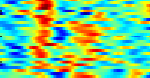
\includegraphics[width=1in]{../figs/avg-eeg.pdf}}};
    \node[boxed] (f0) at (-0.4,1.1) {\phantom{pd}};
    \node[boxed] (f1) at (-0.3,0.9) {\phantom{pd}};
    \node[boxed] (f2) at (-0.2,0.7) {\phantom{pd}};
    \node[boxed] (f3) at (-0.1,0.5) {\phantom{pd}};
    \node[boxed] (f4) at (0.0,0.3) {\phantom{pd}};
    \node[boxed] (f5) at (0.15,0.1) {\phantom{p}continuant\phantom{d}};
    \node[boxed] (f6) at (0.45,-0.4) {\phantom{p}sonorant\phantom{d}};
    \node[boxed] (f7) at (0.75,-0.9) {aspirated};
    \draw[->, thick] (-3.25,0) -- (-2,0);
    \draw[->, thick] (2,0) -- (3,0);
    \node[text width=1in, text centered] (label2) at (4.5,0) {\baselineskip=8pt Foreign phone misperception probabilities};
  \end{tikzpicture}\\
\end{center}
\setlength{\abovecaptionskip}{0pt}
  \caption{EEG responses are recorded while listeners hear speech in
    their native language.  For each listener, a bank of distinctive
    feature classifiers are trained.  Listeners then hear speech in an
    unfamiliar language, and their EEG responses are classified,
    estimating a listener-language probabilistic transcription of the
    non-native speech.}
  \label{fig:eeg_paradigm}
\end{figure}
